\chapter{Implementación}
\label{capitulo5}
\lhead{Capítulo 5. \emph{Implementación}}


\section{Introducción}
El objetivo de este capítulo es explicar detalladamente la implementación realizada en este trabajo.
\clearpage



\section{Descripción general}\label{seccion-corte}

La estimación de odometría por medio de la fusión visual inercial fue desarrollada utilizando C++ como lenguaje de programación y ROS para la aplicación de los filtros inerciales y la visualización del movimiento del robot. Este programa utiliza un sólo hilo de ejecución, de forma que la odometría se estima de forma secuencial, pasando primero por estimar la orientación del robot utilizando el filtro inercial, y luego a estimar la traslación a partir de los residuales inerciales y la cámara. El formato de entrada de las imágenes y de los datos de la IMU fueron tomados de acuerdo al formato empleado en el EUROC Mav dataset.

En cuanto al dataset local realizado, también fue implementado utilizando C++ como lenguaje de programación, y utilizando una raspberry pi 3 para la adquisición de los datos de la imu y de la cámara, y utilizando 4 hilos de ejecución.


\section{Estimación de los residuales rotacionales}

Con el empleo de la IMU es posible obtener los cambios de orientación de la cámara y de su aceleración, siempre y cuando se encuentren sincronizadas las mediciones. Bajo esta restricción se tiene el residual de orientación de la IMU (${R}_{RES/IMU}$) , el cual representa el cambio de orientación de la IMU entre el frame actual y el anterior, tal como se presenta en la ecuación \ref{eq:residualIMU}.


\begin{equation}
{ R }_{ IMU2 }\quad =\quad { R }_{ IMU1 }*{ R }_{ RES/IMU }\quad \rightarrow \quad { R }_{ RES/IMU }\quad =\quad { { { R }_{ IMU1 } }^{ T }*\quad R }_{ IMU2 }
\label{eq:residualIMU} 
\end{equation}

De forma análoga, el residual de la cámara viene dado por:

\begin{equation}
{ R }_{ RES/CAM }\quad =\quad \quad { { R }_{ CAM1 } }^{ T }\quad .\quad { R }_{ CAM2 }
\label{eq:residualCAM} 
\end{equation}

Utilizando la ecuación \ref{eq:rotacionIMUCAM} en \ref{eq:residualCAM}, y las propiedades de la transpuesta del producto de matrices se tiene:

\begin{align}
{ R }_{ RES/CAM }\quad =\quad { { R }_{ CAM1 } }^{ T }.{ R }_{ CAM2 }\quad =\quad ({ R }_{ IMU1 }.{ R }_{ IMU-CAM })\quad ^{ T }.{ R }_{ IMU2 }.{ R }_{ IMU-CAM }\\ \quad \quad \quad \quad \quad \quad \quad \quad \quad =\quad ({ { R }_{ IMU-CAM } }^{ T }.{ { R }_{ IMU1 } }^{ T\quad  })\quad { R }_{ IMU2 }.{ R }_{ IMU-CAM }\\ \qquad \qquad \qquad ={ { \quad R }_{ IMU-CAM } }^{ T }.({ { R }_{ IMU1 } }^{ T\quad  }.{ R }_{ IMU2 }).{ R }_{ IMU-CAM }\\ \qquad \qquad \qquad =\quad { { R }_{ IMU-CAM } }^{ T }.({ { R }_{ IMU1 } }^{ T\quad  }.{ R }_{ IMU2 }).{ R }_{ IMU-CAM }
\label{eq:residualCAMProcedimiento} 
\end{align}

Y finalmente se obtiene:

\begin{equation}
{ R }_{ RES/CAM }\quad =\quad { { \quad R }_{ IMU-CAM } }^{ T }. { R }_{ RES/IMU } . { R }_{ IMU-CAM\\  }
\label{eq:residualCAMDeIMU} 
\end{equation}

De esta forma, utilizando la ecuación \ref{eq:residualCAMDeIMU}, es posible obtener el residual de orientación de la cámara directamente del residual de orientación de la imu.


\section{Estimación de los residuales traslacionales}


En general, en base a las transformaciones de cuerpo rígido se tiene:

\begin{equation}
\left[ \begin{matrix} { X }_{ 1 } \\ { Y }_{ 1 } \\ { Z }_{ 1 } \end{matrix} \right] \quad =\quad { R }_{ 1 }^{ 2 }.\left[ \begin{matrix} { X }_{ 2 } \\ { Y }_{ 2 } \\ { Z }_{ 2 } \end{matrix} \right] +{ P }_{ 1 }^{ 2 } 
\label{eq:TransformacionCAM1CAM2} 
\end{equation}


Donde $(X1, Y1, Z1)$ y $(X2, Y2, Z2)$ representan la ubicación en el espacio del punto característico detectado en la primera y segunda imagen, respectivamente, referidos a cada uno de los sistemas de referencia de la cámara cuando fue tomada la imagen. Utilizando la ecuación \ref{eq:ReproyeccionCAM} se obtiene:


\begin{equation}
{ Z }_{ 1 }\left[ \begin{matrix} \frac { u_{ 1 }-{ c }_{ x } }{ { f }_{ x } }  \\ \frac { { v }_{ 1 }-{ c }_{ y } }{ { f }_{ y } }  \\ 1 \end{matrix} \right] =\quad { R }_{ 1 }^{ 2 }.{ Z }_{ 2 }\left[ \begin{matrix} \frac { u_{ 2 }-{ c }_{ x } }{ { f }_{ x } }  \\ \frac { { v }_{ 2 }-{ c }_{ y } }{ { f }_{ y } }  \\ 1 \end{matrix} \right] +{ P }_{ 1 }^{ 2 }
\label{eq:TransformacionCAM1CAM2Reproyeccion} 
\end{equation}

Debemos recordar que a los puntos de la forma $s (X, Y, Z)$, donde $s$ es un factor de escala, le corresponden el mismo pixel de $(u,v)$ de proyección en la imagen de la cámara. Por tanto, la ecuación \ref{eq:TransformacionCAM1CAM2Reproyeccion} implica que incluso teniendo como medidas los valores de la ubicación  $(u1,v1)$ y $(u2,v2)$ de la ubicación de la pareja de puntos característicos, y conociendo la matriz de rotación ${ R }_{ 1 }^{ 2 }$, que representa el cambio de orientación de la cámara de la imagen 1 a la imagen 2, no es posible determinar la traslación real de la cámara ${ P }_{ 1 }^{ 2 }$, excepto por un factor de escala, sin conocer la profundidad $Z1$ o $Z2$ de la ubicación en el espacio de la característica.


\section{Selección de keyframes}

La implementación de keyframes se hace debido a que la estimación de movimiento es más precisa cuando se tiene disparidad entre las imagenes, y debido a que la carga computacional es menor en procesar un numero selecto de imágenes que la totalidad de ellas.

En este trabajo, los keyframes son seleccionados cuando la disparidad entre las imágenes excede un valor fijo (threshold). Debido a que se cuenta con la información rotacional proveniente del filtro de la IMU, la disparidad es dividida en dos tipos de disparidad: La disparidad traslacional, y la disparidad rotacional.


\subsection{Disparidad rotacional}
La disparidad rotacional es obtenida directamente de los residuales rotacionales entre dos imágenes provenientes del filtro de la IMU, y denotados en la representación RPY, de la siguiente forma:

\begin{equation}
{ D }_{ rot }\quad =\quad \sqrt { { \Delta \phi  }^{ 2 }+{ \Delta \theta  }^{ 2 }+{ \Delta \psi  }^{ 2 }\quad  }
\label{eq:disparidadRotacional}
\end{equation}

Donde ${\Delta \psi}$ es el residual en Yaw, ${\Delta \phi}$ es el residual en Roll, y ${\Delta \theta}$ es el residual en Pitch.

Por tanto, la disparidad rotacional tiene unidades de rad/s ó DPS.


\subsection{Disparidad traslacional}

Por su parte, la disparidad traslacional corresponde al promedio de la distancia euclidiana entre las parejas de las imágenes , expresada en pixeles, resultantes del movimiento traslacional. 


Para obtener la disparidad traslacional es necesario realizar una reproyección de las parejas utilizando sólo la información del residual rotacional. Esto implica que si determinamos la matriz de rotación entre las poses de la cámara en la imagen 1 y 2, y reproyectamos la ubicación de la característica en la imagen 2, hacia la imagen 1, utilizando solo la transformación rotacional, la distancia euclidiana entre la ubicación de la reproyección y la ubicación real del punto característico en la imagen 1, estará vinculada al cambio de traslación de la cámara y la profundidad de las puntos característicos respecto al sistema de referencia de la cámara.
Además, los puntos que se encuentran a mayor distancia de la cámara tendrán mayor distancia euclidiana que los puntos que se encuentren cercanos, para una mismo movimiento de traslación. Esto implica que es posible utilizar esta distancia euclidiana como una medida de la disparidad entre las imágenes producto del movimiento rotacional siempre y cuando se tome alguna forma de restar peso a la profundidad de las características. Es por esto, que tomamos el promedio de la distancia euclidianas entre la reproyección y la ubicación de las características como medida de disparidad entre las imágenes:

\begin{equation}
{ D }_{ tras }\quad =\quad \frac { \sum { \sqrt { ({ u }_{ 1 },\quad { v }_{ 1 })\quad -\quad { rep }_{ { R }_{ 1 }^{ 2 }\quad  }({ u }_{ 2 },\quad { v }_{ 2 }) }  }  }{ N } 
\label{eq:DisparidadTraslacional}
\end{equation}

Donde N es el número de parejas entre las dos imágenes y ${ rep }_{ { R }_{ 1 }^{ 2 }\quad  }({ u }_{ 2 },\quad { v }_{ 2 })$ es la función que reproyecta el punto característico de la imagen 2 en la imagen 1 utilizando la información rotacional ${ R }_{ 1 }^{ 2}$. 
%Por lo tanto el procedimiento es el siguiente
Por tanto, la disparidad traslacional tiene unidades de píxeles.



\section{Estimación de la traslación}

El método para estimar la traslación está basado en una modificación del esquema RANSAC de dos puntos implementado en [].
 
Este método aprovecha la información rotacional y la geometría epipolar para hallar el vector de traslación entre las dos imágenes.

En primer lugar se desea estimar el vector de traslación entre la imagen 1 y la imagen 2.

Se definen los vectores unitarios como:
\begin{equation}
\overset { \rightarrow  }{ { f }_{ i } } =\quad \left[ \begin{matrix} \frac { u_{ i }-{ c }_{ x } }{ { f }_{ x } }  \\ \frac { { v }_{ i }-{ c }_{ y } }{ { f }_{ y } }  \\ 1 \end{matrix} \right] 
\end{equation}





%Robust Real-Time Visual Odometry
%with a Single Camera and an IMU


\subsubsection*{Espacio de color CIELAB}

Conocido en ocasiones con el nombre de l*a*b, es un espacio derivado del \textit{CIE 1931 XYZ}, creado por la comisión internacional de la iluminación CIE (del francés: Comission Internationale de l'Éclairage).

\begin{figure}[h]
	\centering     %%% not \center
	\subfigure[]{\label{fig:lab-a}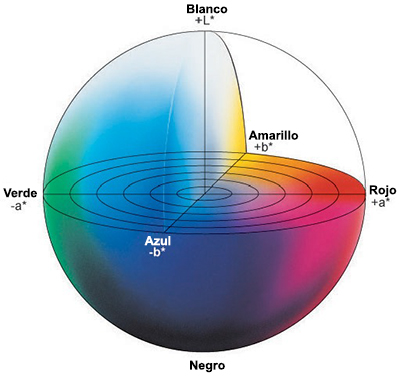
\includegraphics[width=.42\textwidth]{lab1}}
	\subfigure[]{\label{fig:lab-b}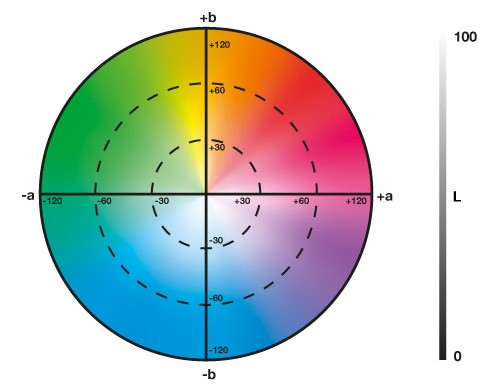
\includegraphics[width=.50\textwidth]{lab2}}
	
	\caption[Espacio de color CIELAB]{Espacio de color CIELAB. En (a) se aprecia el diagrama tridimensional, mientras que en (b) una vista superior del rango de colores con luminancia fija.}
	\label{imagen:lab-color}
\end{figure}

Este es un espacio de color tridimensional descrito por los ejes $a$, que extiende desde verde ($-a$) hasta rojo ($+a$), el eje $b$ que se extiende desde azul ($-b$) hasta amarillo ($+b$), y la luminancia $l$ que varia desde negro ($-l$) hasta blanco ($+l$). Esta representación se puede observar en la figura \ref{imagen:lab-color}.

Debido a que la cantidad de valores para representar los colores en este espacio es menor que en RGB, es mas rápido hacer correcciones de color en LAB, ya que un cambio en la cantidad de valor de una variable produce un cambio con importancia visual. Además de permitir trabajar la iluminación de la imagen por separado de los colores.

\subsection{Método de Reinhard}
El objetivo de esta transformación de color es lograr que la distribución de los puntos en el espacio de color LAB se transfieran entre imágenes. Para esto se utiliza la información de la media y desviación estándar sobre cada canal (L, A y B).

Para un par de imágenes $I$ e $I^*$, donde $I$ es la imagen origen e $I^*$ es la imagen que se quiere corregir, se calcula la media y desviación estándar para cada canal.
\begin{align*}
&{\langle l \rangle} \hspace{0.55cm} {\langle l^* \rangle}  &{ \sigma_l } \hspace{0.5cm} { \sigma^*_l } \\
&{\langle a \rangle} \hspace{0.48cm} {\langle a^* \rangle}  &{ \sigma_a } \hspace{0.5cm} { \sigma^*_a }  \\
&{\langle b \rangle} \hspace{0.5cm} {\langle b^* \rangle}  &{ \sigma_b } \hspace{0.5cm} { \sigma^*_b } 
\end{align*}
Luego se ajusta la distribución de la imagen objetivo restandole la media obtenida en el paso anterior:
\begin{align*}
l^* &= l^* - \langle l^* \rangle \\
a^* &= a^* - \langle a^* \rangle \\
b^* &= b^* - \langle b^* \rangle
\end{align*}
Luego se escalan los valores en función a las desviaciones estándar:
\begin{align*}
l^* &= \frac{\sigma^*_l}{\sigma_l} l^* \\
a^* &= \frac{\sigma^*_a}{\sigma_a} a^* \\
b^* &= \frac{\sigma^*_b}{\sigma_b} b^*
\end{align*}
Finalmente se le suma la media, pero en este caso de la imagen de origen (imagen del color deseado):
\begin{align*}
l^* &= l^* + \langle l \rangle \\
a^* &= a^* + \langle a \rangle \\
b^* &= b^* + \langle b \rangle
\end{align*}
Para lograr un mapeo de color correcto es necesario obtener la información de desviación estándar y media únicamente en el área de intersección entre las imágenes $I\cap I^*$. De esta forma se logra igualar estas regiones de la imagen que deben corresponder a la misma escena.


\section{Fusión de imágenes}\label{seccion-fusion}

Una vez se logra determinar la mejor linea de corte y aplicar una corrección de color, es posible que aun se cuenten con transiciones entre imágenes con cierto nivel de discontinuidad. En este caso es conveniente aplicar algoritmos que permitan una transición suavizada entre dichos bordes.

Se tienen varias versiones de estos algoritmos que serán explicados a continuación: fusión ponderada simple o bajo un esquema piramidal.

\subsection{Fusión ponderada} \label{feathering}
Este tipo de algoritmos realiza una fusión que consiste en realizar un suma ponderada, en la cual se modifica el peso de los píxeles en función de la distancia con el borde de su imagen. Es decir, se realiza una suma de los valores de las imágenes ($\mathtt{I_1},\, \mathtt{I_2}$) en el área de intersección ($\mathtt{I_1}\cap \mathtt{I_2}$) para cada canal, dándole menor peso a los píxeles que se encuentren mas cercanos del extremo de la imagen. Cabe destacar que esta suma se normaliza para asegurar que no se supere el rango $0-255$ con el cual se representan los valores de la imagen final. La ecuación para la suma ponderada se muestra a continuación:
\begin{displaymath}
	F = (1-\alpha)\cdot \mathtt{I}_1 + \alpha\cdot \mathtt{I}_2
\end{displaymath} 
Donde el parámetro $\alpha$ varia en el rango $0\to 1$, en este caso en función a la distancia, tal y como se ilustra en la figura.




El algoritmo de fusión ponderada bajo el esquema de transición presenta ciertas desventajas, entre estas el efecto fantasma, en el que se observan duplicados de los objetos en la escena pero con cierto grado de desvanecimiento. Aunque no será implementado, el estudio de su funcionamiento es necesario para comprender el algoritmo de fusión que trabaja bajo un esquema piramidal.

\subsection{Fusión ponderada piramidal}

El método planteado anteriormente propone una transición suavizada para imágenes que tengan una región en común, presentando así una primera aproximación al problema aquí planteado, sin embargo los algoritmos que se pretenden utilizar en etapas previas (linea de corte) eliminan ésta área de intersección, quedando don imágenes con solo un borde en común. 

Esta técnica es llamada fusión piramidal o fusión multibanda, y su proceso consiste en fusionar las imágenes para distintos niveles de escala. Refiriéndonos a la figura \ref{imagen:piramidal1}, se crea para una misma imagen distintos niveles de escala ($G_i$), donde cada nivel corresponde con una reducción a un cuarto del área del nivel anterior. La cantidad de niveles en la pirámide corresponde con la cantidad de bandas que se quieren fusionar. Es importante mencionar que el proceso de compresión y posterior expansión de una imagen, se aproxima al proceso de aplicar un filtro gaussiano, con lo cual a cada nivel creado $G_i$ recibe el nombre de gaussiana, resultando lo que se denomina una pirámide de gaussianas, tal y como se ilustra en la figura \ref{imagen:piramidal1} con 5 niveles.

\begin{figure}[h]
	\centering
	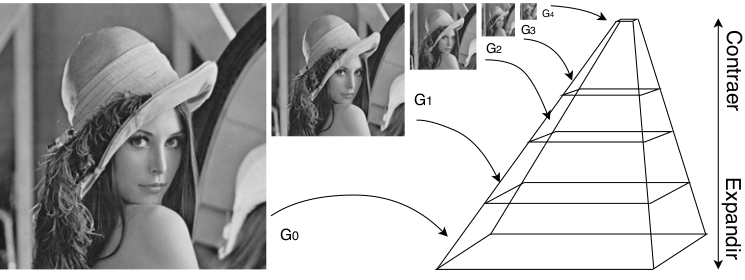
\includegraphics[width=.8\linewidth]{piramidal1.pdf}
	\caption[Construcción de pirámide de gaussianas]{Construcción de pirámide de gaussianas}
	\label{imagen:piramidal1}
\end{figure}

\begin{figure}[h]
	\centering
	\includegraphics[width=.8\linewidth]{piramidal2.pdf}
	\caption[Construcción de pirámide de laplacianas]{Construcción de pirámide de laplacianas}
	\label{imagen:piramidal2}
\end{figure}

Una vez se tiene la pirámide de gaussianas, se elabora una pirámide de laplacianas utilizando \textit{DoG}, es decir, cada nivel de esta pirámide se construye restando un nivel de la pirámide gaussiana con su nivel siguiente pero expandido (para lograr las mismas dimensiones). Al restar una imagen con ella misma pero aplicada un filtro gaussiano --- que remueve las componentes en bajas frecuencias ---, se logra una imagen que resalte las componentes en las frecuencias altas. Esta composición se puede observar en la figura \ref{imagen:piramidal2}, donde a cada imagen laplaciana $L_i$ se le sumó una constante para efectos de visualización, ya que presenta valores muy bajos al aplicar únicamente la resta.

Como ya se mencionó, este proceso se aplica para imágenes que no comparten un área de superposición, con lo cual es necesario definir mediante una máscara binaria los límites de cada imagen. Convenientemente, el proceso de determinar la línea de corte ya nos ofrece esta máscara mediante el proceso de etiquetado, con lo cual se utiliza para definir las fronteras en esta fusión.

La pirámide gaussiana que se elaboró en un principio para cada imagen a fusionar, debe también crearse para la máscara, ya que la fusión debe realizarse en cada nivel de la pirámide. Finalmente para mostrar la imagen final en la resolución original, el proceso de fusión debe realizarse escalando cada nivel hasta las dimensiones originales.

Éste proceso consiste en expandir el último nivel de la pirámide --- con su respectiva máscara---, una vez expandido se le suma el laplaciano correspondiente, devolviéndole la componente en alta frecuencia que le fue removida. En este punto se tiene el par de imágenes expandidas un nivel, además de la máscara aun afectada por el efecto del filtro gaussiano, con lo cual se efectúa una suma ponderada entre las dos imágenes similar que en la sección \ref{feathering}, pero en este caso se utiliza la máscara difuminada para determinar el peso de la suma, y donde el inverso de la máscara determina la ponderación de la segunda imagen.

En la figurase puede observar el resultado de aplicar una fusión bajo el esquema piramidal.


%%%%%%%%%%%%%%%%%%%%%%%%%%%%%%%%%%%%%%%%%%%%%%%%%%%%%%%%%%%%%%%%%%%%%%%%%%%%%%%
\section{Resultados}


Hasta ahora se han presentado casos en los que se lidia con un par de imágenes. Por lo tanto se presenta un mosaico compuesto por tres imágenes del conjunto \textit{Espenky}, adicionalmente se tiene un error producido por el efecto paralaje. En este caso el algoritmo busca por la mejor linea de corte para cada par de imágenes por separado, pero logrando un mosaico final sin errores de discontinuidades.

En este ejemplo en particular se logra evidenciar una debilidad que tiene este algoritmo. A pesar de ser muy robusto al evadir objetos por la diferencia de texturas y bordes, es común que se cuente con discontinuidades visuales producto de cambios de iluminación.


\section{Resumen}

En esta sección se presentan los errores resultantes de las etapas de alineación, y que evitan que se logre un  mosaico que cumpla con el objetivo de aparentar ser una misma imagen. Luego del planteamiento del problema se exponen y describen distintos algoritmos que buscan una solución a estos.

En su mayoría estos algoritmos buscan reducir las discontinuidades entre imágenes producto de objetos en movimiento dentro de la escena, errores de alineación de objetos y texturas, y diferencias de iluminación. Al final del capítulo se presentaron los distintos resultados que muestran la efectividad de los algoritmos descritos, en primer lugar resultados concretos de los módulos por separado y finalmente con resultados de mosaicos completos de los conjunto de datos estudiados, aplicando para estos el sistema completo especificado al inicio del presente proyecto.

